\documentclass[12pt]{article}
\usepackage{amsmath}
\usepackage{times}
\usepackage{graphicx}
\usepackage{color}
\usepackage{multirow}
%
\usepackage[authoryear]{natbib}
%
\usepackage{rotating}
\usepackage{bbm}
\usepackage{latexsym}
%
\usepackage{tikz}
\usetikzlibrary{shapes.geometric, arrows}

%%% margins 
\textheight 23.4cm
\textwidth 14.65cm
\oddsidemargin 0.375in
\evensidemargin 0.375in
\topmargin  -0.55in
%
\renewcommand{\baselinestretch}{2}
%
\interfootnotelinepenalty=10000
%
\renewcommand{\thesubsubsection}{\arabic{section}.\arabic{subsubsection}}
\newcommand{\myparagraph}[1]{\ \\{\em #1}.\ \ }
\newcommand{\citealtt}[1]{\citeauthor{#1},\citeyear{#1}}
\newcommand{\myycite}[1]{\citep{#1}}

% Different font in captions
\newcommand{\captionfonts}{\normalsize}

\makeatletter  
\long\def\@makecaption#1#2{%
  \vskip\abovecaptionskip
  \sbox\@tempboxa{{\captionfonts #1: #2}}%
  \ifdim \wd\@tempboxa >\hsize
    {\captionfonts #1: #2\par}
  \else
    \hbox to\hsize{\hfil\box\@tempboxa\hfil}%
  \fi
  \vskip\belowcaptionskip}
\makeatother   
%%%%%

\renewcommand{\thefootnote}{\normalsize \arabic{footnote}} 	

% Declare useful math operators
\DeclareMathOperator*{\argmin}{arg\,min}
\DeclareMathOperator*{\plim}{plim}
\DeclareMathOperator{\Tr}{Tr}
\begin{document}
\hspace{13.9cm}1

\ \vspace{20mm}\\

{\LARGE Heterogeneous synaptic weighting improves neural coding under the presence of common noise}

\ \\
{\bf \large Pratik S. Sachdeva$^{\displaystyle 1, \displaystyle 2}$, Michael R. DeWeese$^{\displaystyle 1, \displaystyle 2}$}\\
{$^{\displaystyle 1}$Redwood Center for Theoretical Neuroscience.}\\
{$^{\displaystyle 2}$University of California, Berkeley.}\\
%

%\ \\[-2mm]
{\bf Keywords:} neural variability, noise correlations, shared and private noise, synaptic weighting

\thispagestyle{empty}
\markboth{}{NC instructions}
%
\ \vspace{-0mm}\\
%
%Abstract
\begin{center} {\bf Abstract} \end{center}
This documentation briefly describes the formats required by Neural Computation. We hope this will help you with the manuscript preparation.
%%%%%%%%%%%

\section{Introduction}
Variability is a prominent feature of neural systems: neural responses to external stimuli will vary trial-to-trial even when the stimuli are constant. Furthermore, neural variability exhibits pairwise correlations: these ``noise correlations'' have been observed throughout the cortex. They have long been of theoretical interest because their presence has strong implications for neural coding.

From a population coding perspective, a neural population must produce a faithful representation of relevant quantities, such as a stimulus, for their computation. One advantage of population coding is that variability unique to each neuron, or private variability, can be averaged out. If some variability is shared across neurons, i.e. we have noise correlations, larger populations of neurons cannot naively average out the variability. An abundance of theoretical work has explored how shared variability, therefore, can be both detrimental or beneficial to the fidelity of a population code depending on its structure. A  general conclusion of this theoretical work highlights the importance of the geometric relationship between the signal and noise correlations (both of which are stimulus-dependent).

Thus, the sources of neural variability - and their respective contributions to the private and shared components - will have a significant impact on shaping the geometry of the population's correlational structure, and therefore coding ability. For example, private sources of variability such as channel noise or stochastic synaptic vesicle release could be averaged out by large populations of neurons. But sources of variability shared across neurons - such as the variability of presynaptic spike trains - would induce noise correlations and place different constraints on our neural code.  Indeed, any variability carried by an incoming stimulus possesses would also introduce variability in the population. Such ``shared input noise'' is particularly detrimental to the fidelity of a population code.

In prior work, we examined private and shared variability in the auditory cortex. Specifically, we partitioned sub-threshold variability of a neural populationinto private components (synaptic, thermal, and other local sources of variability) and shared components (variability induced by afferent connections). We found that the private component of the total variability is quite small, while the shared component can be much larger (Figure \ref{fig:private-shared}B). Thus, the large shared component of a neuron's variability, a source of noise correlations, has important consequences for neural coding.

We sought out to explore how shared and private sources of neural variability interact to influence neural coding. As mentioned before, work by Moreno-Bote et al. demonstrated that shared input noise is detrimental to the fidelity of a population code. Here, we instead turn to sources of shared variability which are not carried by stimulus and thus can be manipulated by features of neural computation such as synaptic weighting. We refer to these noise sources as ``common noise'' to distinguish them from the special case of ``shared input noise.'' For example, a common noise source could include an upstream neuron whose action potentials are ``noisy'' in the sense that they are unimportant for the computation of the current stimulus.

We consider a simple linear-nonlinear architecture and explore how its high-dimensional neural representation is impacted by a common noise source, which acts as an input, and private noise variability across all neurons. We chose the simple architecture as it allowed us to analytically assess coding ability through the Fisher and mutual informations. We found surprising cases where synaptic weighting that introduced more noise into our network via the common noise resulted in improved coding performance. Lastly, we found that the amount of private and common variance was vitally important for what types of synaptic weighting resulted in the best performance for the network.
\begin{figure}[t]
	\centering
	\scalebox{0.50}{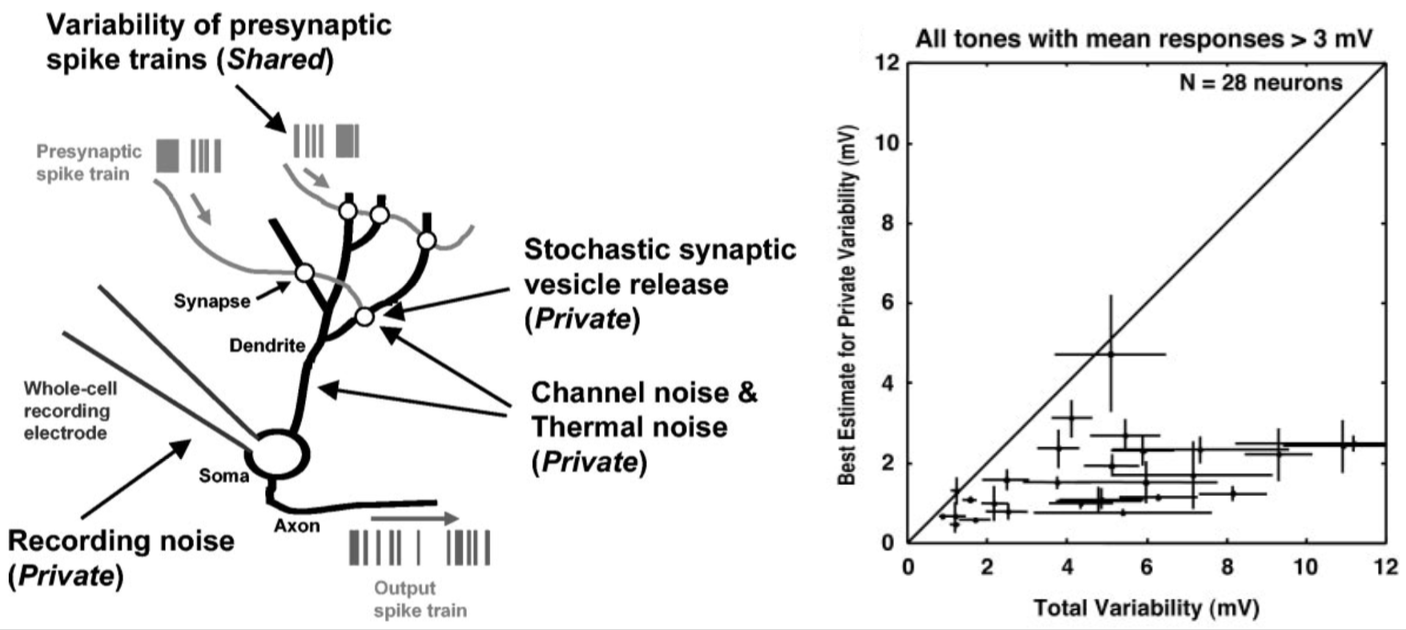
\includegraphics{img/figure1.png}}
	\caption{Shared and private variability. \textbf{(A)} The variability of a neural population contain both private components (e.g. synaptic vesicle release, channel noise, thermal noise, etc.) and shared components (e.g. variability of presynaptic spike trains). Shared variability can be induced by the private variability of afferent connections (which is shared across a postsynaptic population) or inherited from the stimulus itself. \textbf{(B)}} Estimates of the private variability contributions to the total variability of neurons $(N=28)$ recorded from auditory cortex of anesthetized rats. Diagonal line indicates the identity line. Figure reproduced from \cite{deweese2004}.
	\label{fig:private-shared}
\end{figure}

\section{Methods}

\subsection{Network Architecture}
We consider the linear-nonlinear architecture depicted in Figure \ref{architecture}. The inputs to the network consist of a stimulus $s$ along with common (Gaussian) noise $\xi_C$. The $N$ neurons in the network take a linear combination of the inputs which is then corrupted by i.i.d. private Gaussian noise. Thus, the output of the linear stage for the $i$th neuron is 
\begin{align}
\ell_i &= v_i s + w_i \sigma_C \xi_C + \sigma_P\xi_{P,i},
\end{align}
where $\xi_{P,i}$ is the private noise. Both noise terms are scaled by positive constants $\sigma_C$ and $\sigma_P$ in order to make their variances explicit. The noisy linear combination is passed through a nonlinearity $g_i(\ell_i)$ whose output $r_i$ can be thought of as a firing rate. We consider the cases in which $\mathbf{r}$ alone serves as the network's output and when it acts as the mean for a Poisson firing process.

Thus, the network-wide computation is given by
\begin{align}
\mathbf{r} &= \mathbf{g}(\mathbf{v} s + \mathbf{w} \sigma_C \xi_C +\sigma_P \boldsymbol{\xi}_P)
\end{align}
where vector notation denotes the weights, noises, and nonlinearities across the neuronal population. In this scheme the correlational structure of the network is dictated by the choice of weight vectors $\mathbf{v}$, $\mathbf{w}$ along with the array of nonlinearities $\mathbf{g}$. 
\begin{figure}[ht]
	\centering
	\scalebox{1.0}{
		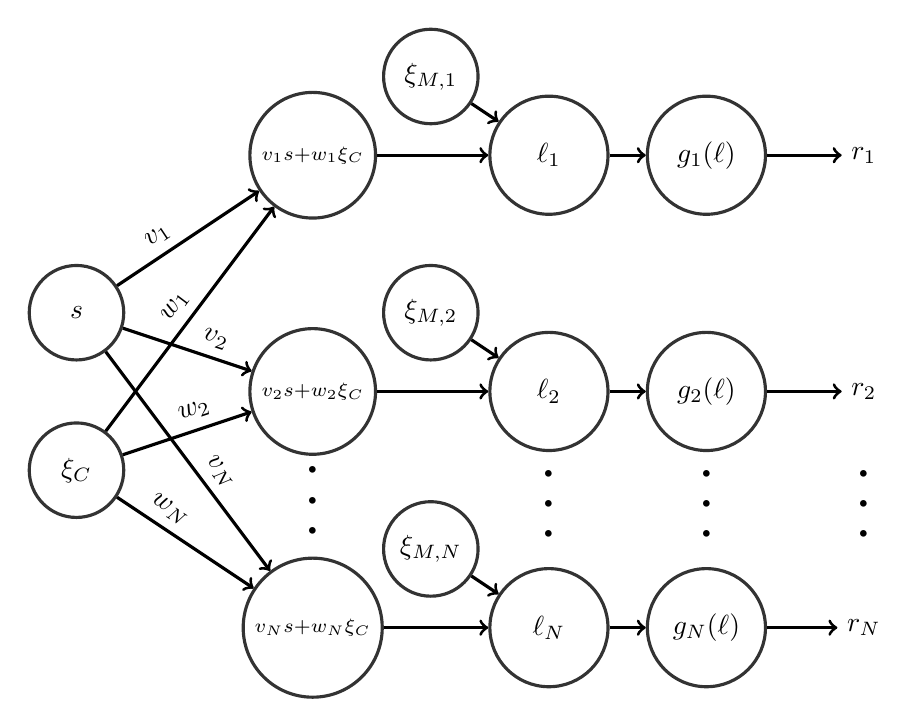
\begin{tikzpicture}
		\tikzstyle{main} = [circle, minimum size = 12mm, line width = 0.4mm, draw=black!80, node distance = 16mm]
		\tikzstyle{main2} = [circle, minimum size = 15mm, line width = 0.4mm, draw=black!80, node distance = 16mm]
		\node[main, fill = white!100] at (-2, 1.) (s) {$s$};
		\node[main, fill = white!100] at (-2, -1.) (common) {$\xi_C$};
		
		\node[main2] at (1.,3.0)  (l1) {${\scriptstyle v_1 s + w_1 \xi_C}$};
		\node[main2] at (1.,0.0)  (l2) {${\scriptstyle v_2 s + w_2 \xi_C}$};
		\node[main2] at (1,-3.0) (lN) {${\scriptstyle v_N s + w_N \xi_C}$};
		
		\node[main2] at (4.,3.0)  (ell1) {$\ell_1$};
		\node[main2] at (4.,0.0)  (ell2) {$\ell_2$};
		\node[main2] at (4,-3.0) (ellN) {$\ell_{N}$};
		
		\node[main2] at (6, 3.0) (nonlin1) {$g_1(\ell)$};
		\node[main2] at (6, 0.0) (nonlin2) {$g_2(\ell)$};
		\node[main2] at (6, -3.0) (nonlinN) {$g_N(\ell)$};
		
		\node at (8, 3.0) (r1) {$r_1$};
		\node at (8, 0.0) (r2) {$r_2$};
		\node at (8, -3.0) (rN) {$r_N$};
		
		\node[main] at (2.5, 4.0) (xi1) {$\xi_{M,1}$};
		\node[main] at (2.5, 1.0) (xi2) {$\xi_{M,2}$};
		\node[main] at (2.5, -2.0) (xiN) {$\xi_{M,N}$};
		
		\draw[->, line width = 0.4mm] (s) -- (l1) node[midway, above left, sloped] {$v_1$};
		\draw[->, line width = 0.4mm] (s) -- (l2) node[midway, above right, sloped] {$v_2$};
		\draw[->, line width = 0.4mm] (s) -- (lN) node[midway, above right, sloped] {$v_N$};
		
		\draw[->, line width = 0.4mm] (common) -- (l1) node[pos = 0.6, above left, sloped] {$w_1$};
		\draw[->, line width = 0.4mm] (common) -- (l2) node[pos = 0.8, above left, sloped] {$w_2$};
		\draw[->, line width = 0.4mm] (common) -- (lN) node[midway, above left, sloped] {$w_N$};
		
		\draw[->, line width = 0.4mm] (l1) -- (ell1);
		\draw[->, line width = 0.4mm] (l2) -- (ell2);
		\draw[->, line width = 0.4mm] (lN) -- (ellN);
		
		\draw[->, line width = 0.4mm] (xi1) -- (ell1);
		\draw[->, line width = 0.4mm] (xi2) -- (ell2);
		\draw[->, line width = 0.4mm] (xiN) -- (ellN);
		
		\draw[->, line width = 0.4mm] (ell1) -- (nonlin1);
		\draw[->, line width = 0.4mm] (ell2) -- (nonlin2);
		\draw[->, line width = 0.4mm] (ellN) -- (nonlinN);
		
		\draw[->, line width = 0.4mm] (nonlin1) -- (r1);
		\draw[->, line width = 0.4mm] (nonlin2) -- (r2);
		\draw[->, line width = 0.4mm] (nonlinN) -- (rN);
		
		\path (l2) -- (lN) node [black, font=\Huge, midway, sloped] {$\dots$};
		\path (ell2) -- (ellN) node [black, font=\Huge, midway, sloped] {$\dots$};
		\path (nonlin2) -- (nonlinN) node [black, font=\Huge, midway, sloped] {$\dots$};
		\path (r2) -- (rN) node [black, font=\Huge, midway, sloped] {$\dots$};	
		\end{tikzpicture}}
	
	\caption{Linear-Nonlinear Network Architecture. The network takes as its inputs a stimulus $s$ and common noise $\xi_C$. A linear combination of these quantities is corrupted by individual membrane potential noise $\xi_{P,i}$. The output of this linear stage is then passed through a nonlinearity $g_i(\ell)$.}
	\label{architecture}
\end{figure}

\subsection{Measures of Coding Strength}
In order to assess the fidelity of the population code represented by $\boldsymbol{\ell}$ or $\mathbf{r}$, we turn to the Fisher information and the Shannon mutual information. The former has largely been utilized in the context of sensory decoding and correlated variability \citep{abbott1999} while the latter has been well studied in the context of efficient coding. 

The Fisher information sets a limit by which the readout of a population code can determine the value of the stimulus. Formally, it sets a lower bound to the variance of an unbiased estimator for the stimulus. Often, the Fisher information is intractable to calculate analytically; a suitable lower bound is the linear Fisher information:
\begin{align}
I_F(s) &= \mathbf{f}'(s)^T \boldsymbol{\Sigma}^{-1}(s) \mathbf{f}(s)
\end{align}
whose corresponding estimator is the locally optimal linear estimator. 

The Shannon mutual information quantifies the reduction in uncertainty of one random variable given knowledge of another. In the context of Figure \ref{architecture}, we are interested in the mutual information between the neural representation $\mathbf{r}$ and the stimulus $s$, i.e. $I[s, \mathbf{r}]$. As with the Fisher information, the mutual information is often not analytically tractable. Thus, we turn to the abundance of work devoted to formulating estimators of the mutual information from data. Specifically, we will utilize the nearest-neighbor estimator developed by Kraskov et al. 
\subsection{Structured Weights}
To obtain analytic expressions for these quantities, we first consider the case of ``structured weights'' taking on the form
\begin{align}
c \times \left(\underbrace{1 \cdots 1}_{N/k \text{ times}}  \ \underbrace{2 \cdots 2}_{N/k \text{ times}} \ \cdots \ \underbrace{k \cdots k}_{N/k \text{ times}}   \right)^T.
\end{align}
Specifically, the structured weight vectors are parameterized by an integer $k$ which divides the $N$ weights into $k$ homogeneous groups. The weights across the groups span the positive integers up to $k$, and we allow for a final scaling factor $c$. 

Importantly,  larger $k$ will only increase the weights in the vector. Thus, in the above scheme, increased ``diversity'' can only be achieved through an increase through the parameter $k$, which will invariably result in an amplification of the signal to which the weight vector is applied. In the case that $k$ does not evenly divide $N$, the last group is repeated $N\text{mod }k$ times.

Lastly, we will consider cases when $k$ is of the order $N$, e.g. $k = N/2$. Such a value of $k$ ensures that the weights grow with the population size. This is in contrast for $k$ a constant, such as $k=4$, which sets a maximum weight size no matter the population size. 
\subsection{Unstructured Weights}

While the structured weights provide us analytic results, they possess an unrealistic distribution of synaptic weighting. Thus, we turn to the case of ``unstructured weights,'' in which the synaptic weights are drawn from some parameterized probability distribution:
\begin{align}
\mathbf{v} \sim p(\mathbf{v}; \theta_{\mathbf{v}}); \ \mathbf{w} \sim p(\mathbf{w}; \theta_{\mathbf{w}}).
\end{align}
Thus, we  calculate both information theoretic quantities over many random draws from these distributions. We then observe how the quantities behave as some subset of the parameters $\theta$ are varied. In particular, we will focus on the lognormal distribution, which has been observed to describe the distribution of synaptic weights well in slice electrophysiology \textcolor{red}{[citation]}. Specifically, we examine 
\begin{align}
\mathbf{w}\sim \text{Lognormal}(\mu - \Delta, \sigma)
\end{align}
\section{Results}
We consider the network's coding ability after both the linear stage $(\boldsymbol{\ell})$ and the nonlinear stage $(\mathbf{r})$. The linear stage can be considered the output of the network assuming the functions $\mathbf{g}$ are simply the identity. Furthermore, the qualitative conclusions we obtain from the linear stage should apply for any one-to-one nonlinearity. 
	
\subsection{Linear Stage}
\begin{figure}[t]
	\centering
	\scalebox{0.31}{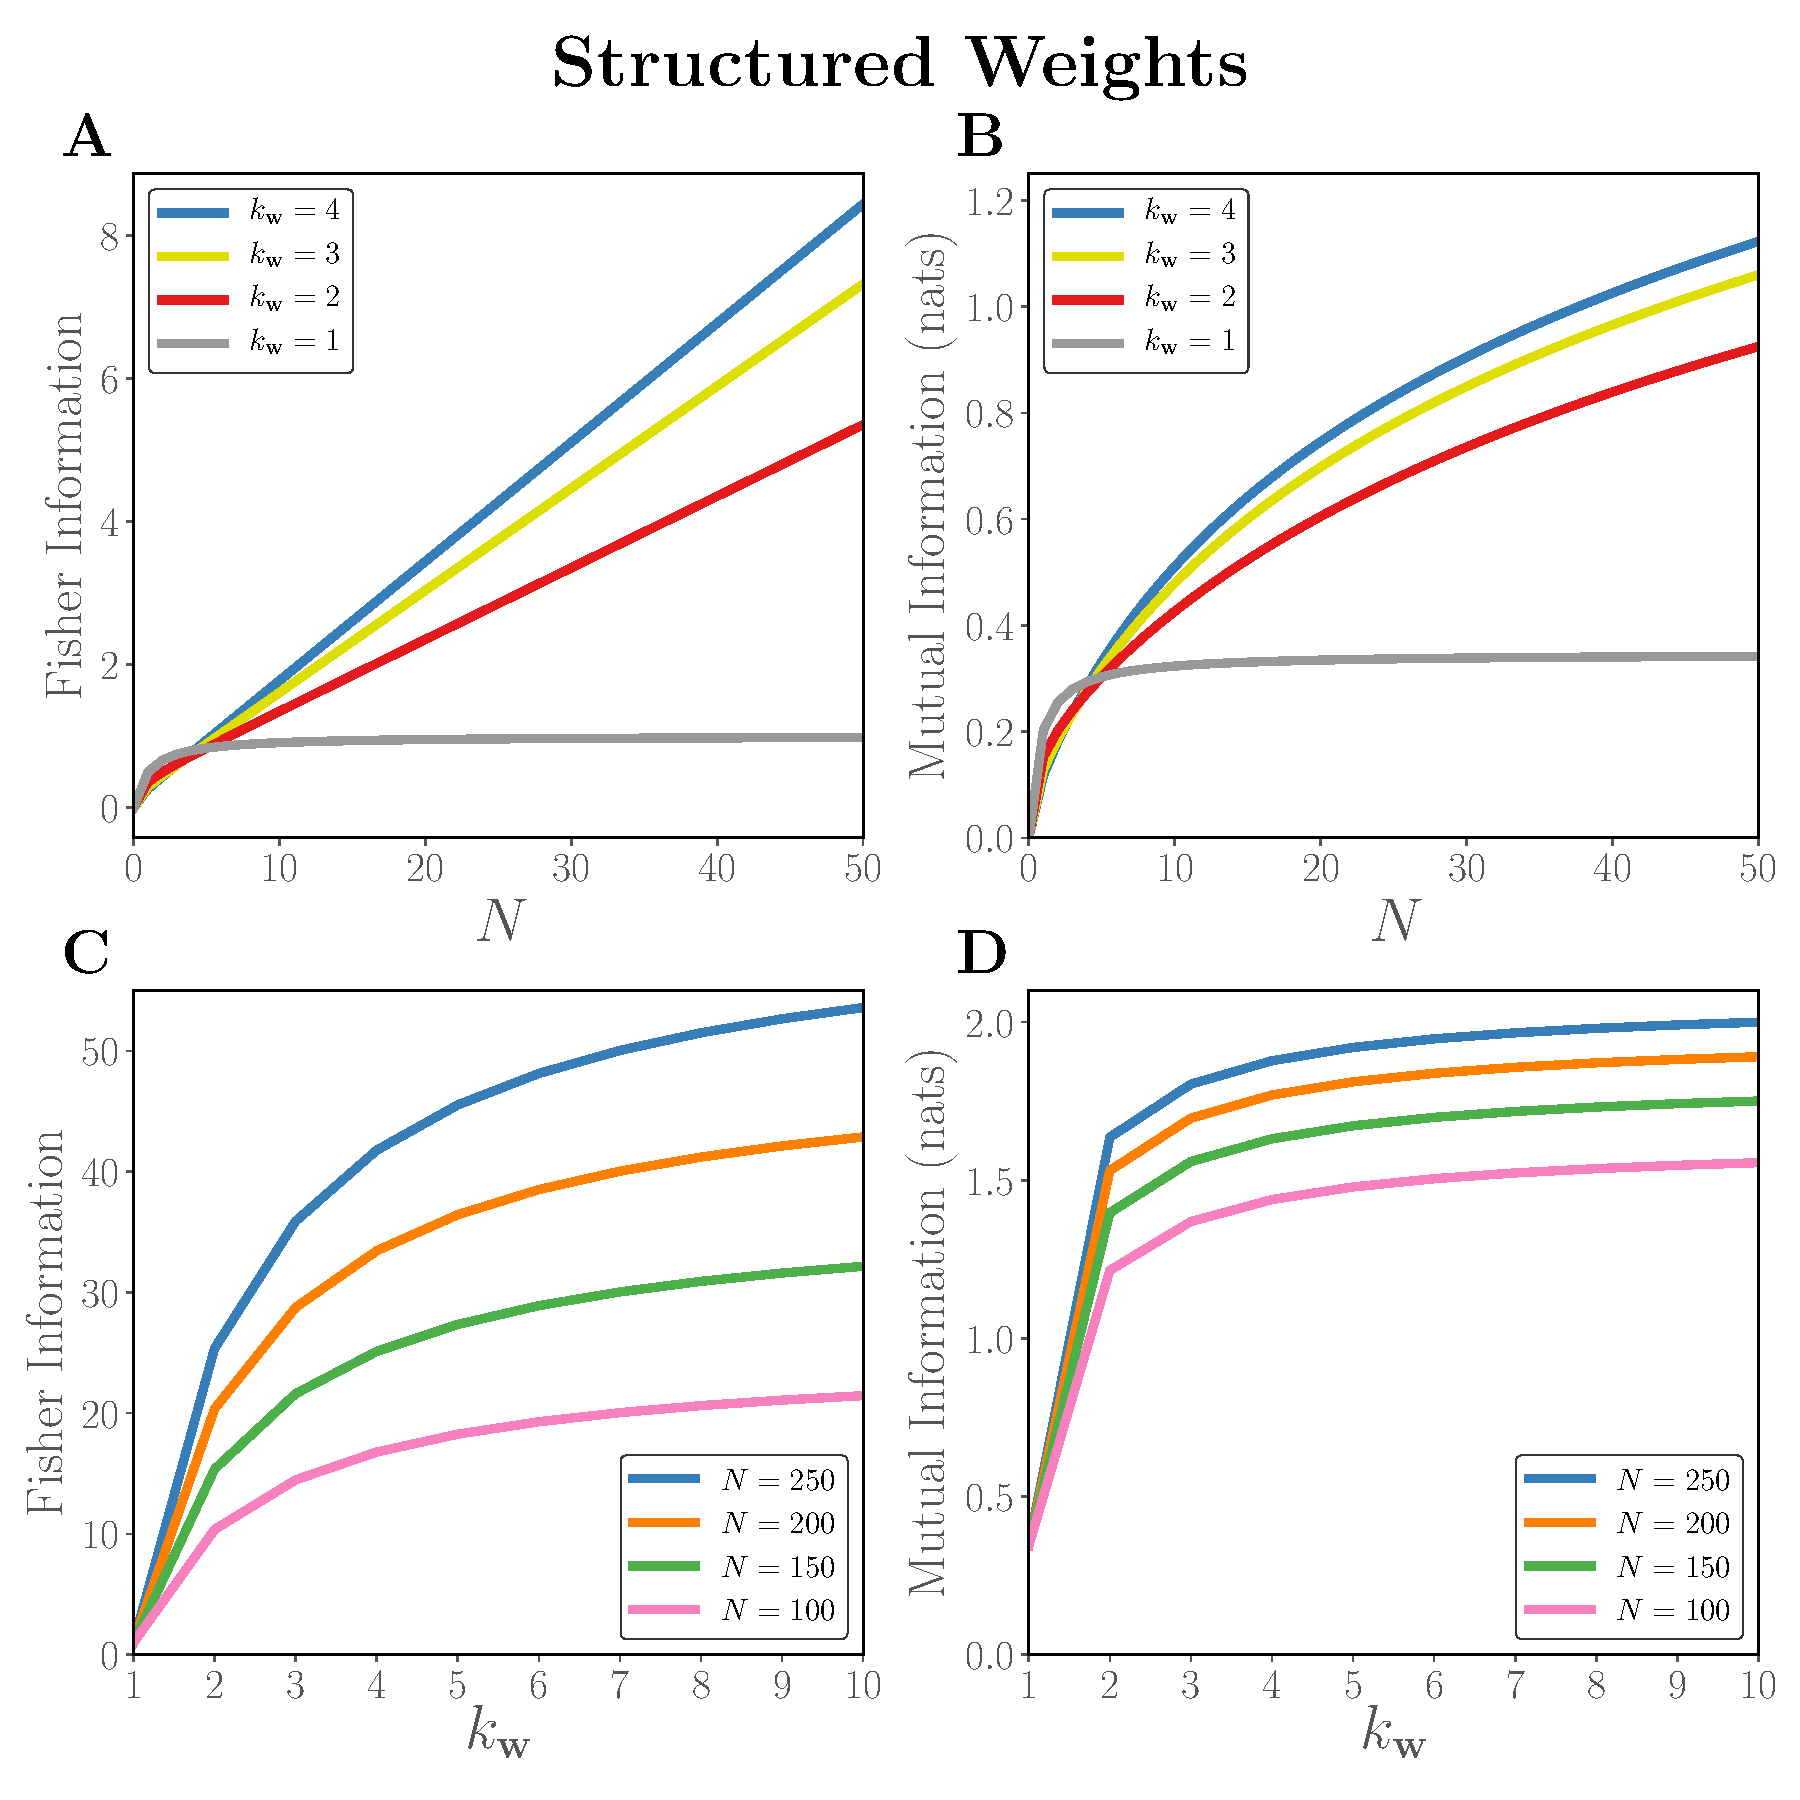
\includegraphics{img/figure2-part1.pdf}}
	\scalebox{0.31}{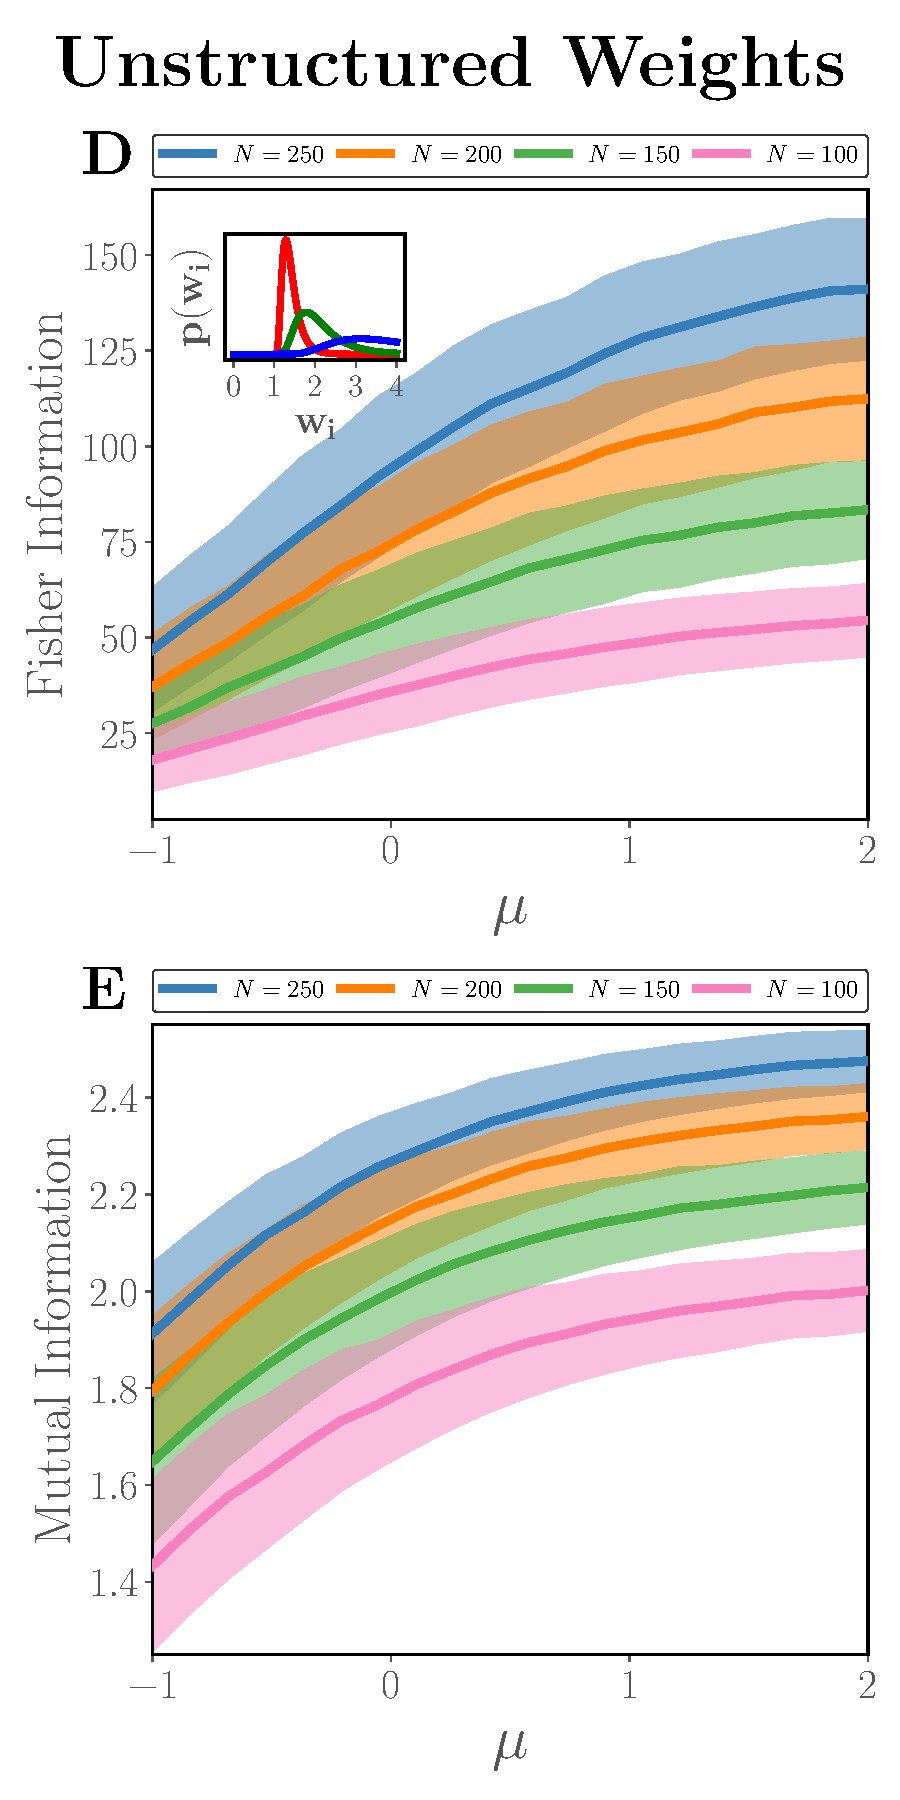
\includegraphics{img/figure2-part2.pdf}}
	\caption{The performance of the Fisher and mutual informations after the linear stage of the network. Here, we take $\sigma_P = \sigma_C=1$. Note that the Fisher information is independent of $s$. \textbf{(A)}, \textbf{(C)} Structured weights. Both quantities saturate as a function of the number of neurons in the case of uniform noise weights ($k_{\mathbf{w}}=1$). Once $k_{\mathbf{w}}$ is increased, they are unbounded with respect to population size. \textbf{(B)}, \textbf{(D)} Same aforementioned network, but plotted with respect to weight heterogeneity for various network sizes. \textbf{(E)}, \textbf{(F)} Unstructured weights calculated over 2000 draws from lognormal distributions. Inset shows the distribution of weights for various choices of $\mu$. Increasing $\mu$ shifts the distribution to the right, increasing heterogeneity. Solid lines depict the means while the shaded region indicate one standard deviation across samples.}\label{fig:struct-linear}
\end{figure}
	
	The Fisher information in the linear representation is calculated in Appendix \ref{app:fisher-linear} as 
	\begin{align}
	I_F(s) &= \frac{1}{\sigma_P^2}\frac{\left(\sigma_P^2/\sigma_C^2\right) |\mathbf{v}|^2 +  \left(|\mathbf{v}|^2|\mathbf{w}|^2 - (\mathbf{v}\cdot\mathbf{w})^2\right)}{(\sigma_P^2/\sigma_C^2)+ |\mathbf{w}|^2}. \label{eqn:fisher-linear}
	\end{align}
	while the mutual information is calculated in Appendix \ref{mutual-linear} as
	\begin{align}
	I[s, \boldsymbol{\ell}] &= \frac{1}{2} \log \left[1 + \sigma_S^2 I_F(s)\right]. \label{eqn:mutual-linear}
	\end{align}
	In the case of mutual information, we have assumed the stimulus prior is Gaussian with zero mean and variance $\sigma_S^2$. For structured weights, equations \ref{eqn:fisher-linear} and \ref{eqn:mutual-linear} can be explored by varying the choice of $k$ for both $\mathbf{v}$ and $\mathbf{w}$ (call them $k_{\mathbf{v}}$ and $k_{\mathbf{w}}$, respectively).
	
	It is simplest to examine these quantities with $k_{\mathbf{v}}=1$ while allowing $k_{\mathbf{w}}$ to vary, as amplifying and diversifying $\mathbf{v}$ will increase coding ability (which our results corroborate) \cite{Ecker2011}. On the other hand, while increasing $k_{\mathbf{w}}$ will boost the overall noise added into the neural population, it also changes the direction that the noise is projected into the higher-dimensional neural space. Thus, while we might expect that more noise in the system would hinder coding, the direction to which the noise is projected is important. 
	
	We first consider how the Fisher information and mutual information are impacted by the choice of $k_{\mathbf{w}}$. In the structured regime, we have 
	\begin{align}
	|\mathbf{v}|^2 &= N \\
	\mathbf{v}\cdot\mathbf{w} &= \frac{N}{k} \sum_{i=1}^k i = \frac{N(k+1)}{2} \\
	|\mathbf{w}|^2 &= \frac{N}{k}\sum_{i=1}^k i^2 = \frac{N(k+1)(2k+1)}{6},
	\end{align}
	which allows us to rewrite equation \ref{eqn:fisher-linear} as
	\begin{align}
	I_F(s) = I_F &= \frac{N}{2\sigma_P^2} \frac{12 (\sigma_P^2/\sigma_C^2) + N  (k^2-1)}{6(\sigma_P^2/\sigma_C^2)+ N(2k^2+3k+1)}.
	\end{align}
	The form of the mutual information follows directly from equation \ref{eqn:mutual-linear}. The structured regime analytically reveals the asymptotic behavior of the information quantities. Both quantities saturate as a function of $N$  only in the case of $k_{\mathbf{w}}=1$ (Figure \ref{fig:struct-linear}A, C); otherwise, they increase without bound. As expected, increasing the population of the system also enhances coding fidelity. Furthermore, both quantities are monotonically increasing functions of $k_{\mathbf{w}}$ (Figure \ref{fig:struct-linear}B, D), implying that encoding and decoding are enhanced despite the fact that the common noise is magnified for larger $k_{\mathbf{w}}$. Our analytic results ensure linear and logarithmic growth for the Fisher and mutual information, respectively, as one might expect in the case of Gaussian noise \cite{Brunel1998}. These qualitative results hold for any choice of $(\sigma_S, \sigma_P, \sigma_C)$.
	
	In the case of $k_{\mathbf{w}}=1$, the signal and common noise are aligned perfectly in the neural representation. Thus, the common noise becomes equivalent in form to shared input noise. As a consequence, we observe the saturation of both Fisher and mutual informations as a function of the neural population. Such saturation implies the existence of differential correlations, consistent with the observation that information-limiting correlations occur under the presence of shared input noise \cite{Moreno-Bote2014}. This does not imply that weight heterogeneity prevents differential correlations, as the common noise in this model is manipulated by synaptic weighting, in contrast with true shared input noise. It does, however, imply that weight heterogeneity can prevent the harmful effects of \textit{additional} information-limiting correlations induced by common noise mimicking shared input noise.
	
	While the structured weights provide us analytic results, they possess an unrealistic distribution of synaptic weighting. Thus, we turn to ``unstructured weights,'' in which the synaptic weights are drawn from a shifted lognormal distribution. In this case, we calculate both information theoretic quantities over many random draws according to $w_i \sim \Delta + \text{Lognormal}(\mu, \sigma^2)$. We are primarily concerned with varying $\mu$, as an increase in this quantity uniformly increases the mean, median, and mode of the lognormal distribution (Figure  \ref{fig:struct-linear}E, inset), akin to increasing $k_{\mathbf{w}}$ for the structured weights. 
	
	Our numerical analysis demonstrates that increasing $\mu$ will increase the average Fisher information and average mutual information for multiple network sizes (Figure \ref{fig:struct-linear}E, F: bold lines). In addition, the benefits of larger weight diversity are felt more strongly by larger populations (Figure \ref{fig:struct-linear}E, F: shaded region). Thus, we once again observe that larger heterogeneity affords the network improved coding performance, despite the increased noise present in the system.
	
	\subsection{Quadratic Nonlinearity}
	We next consider the performance of the network after a quadratic nonlinearity $g_i(x) = x^2$ for all neurons $i$. In this case, both the Fisher information and mutual information are analytically intractable. Thus, we will instead turn to the linear Fisher information (which is feasible) and approximate the mutual information numerically.
	
	\begin{figure}[t]
		\centering
		\scalebox{0.23}{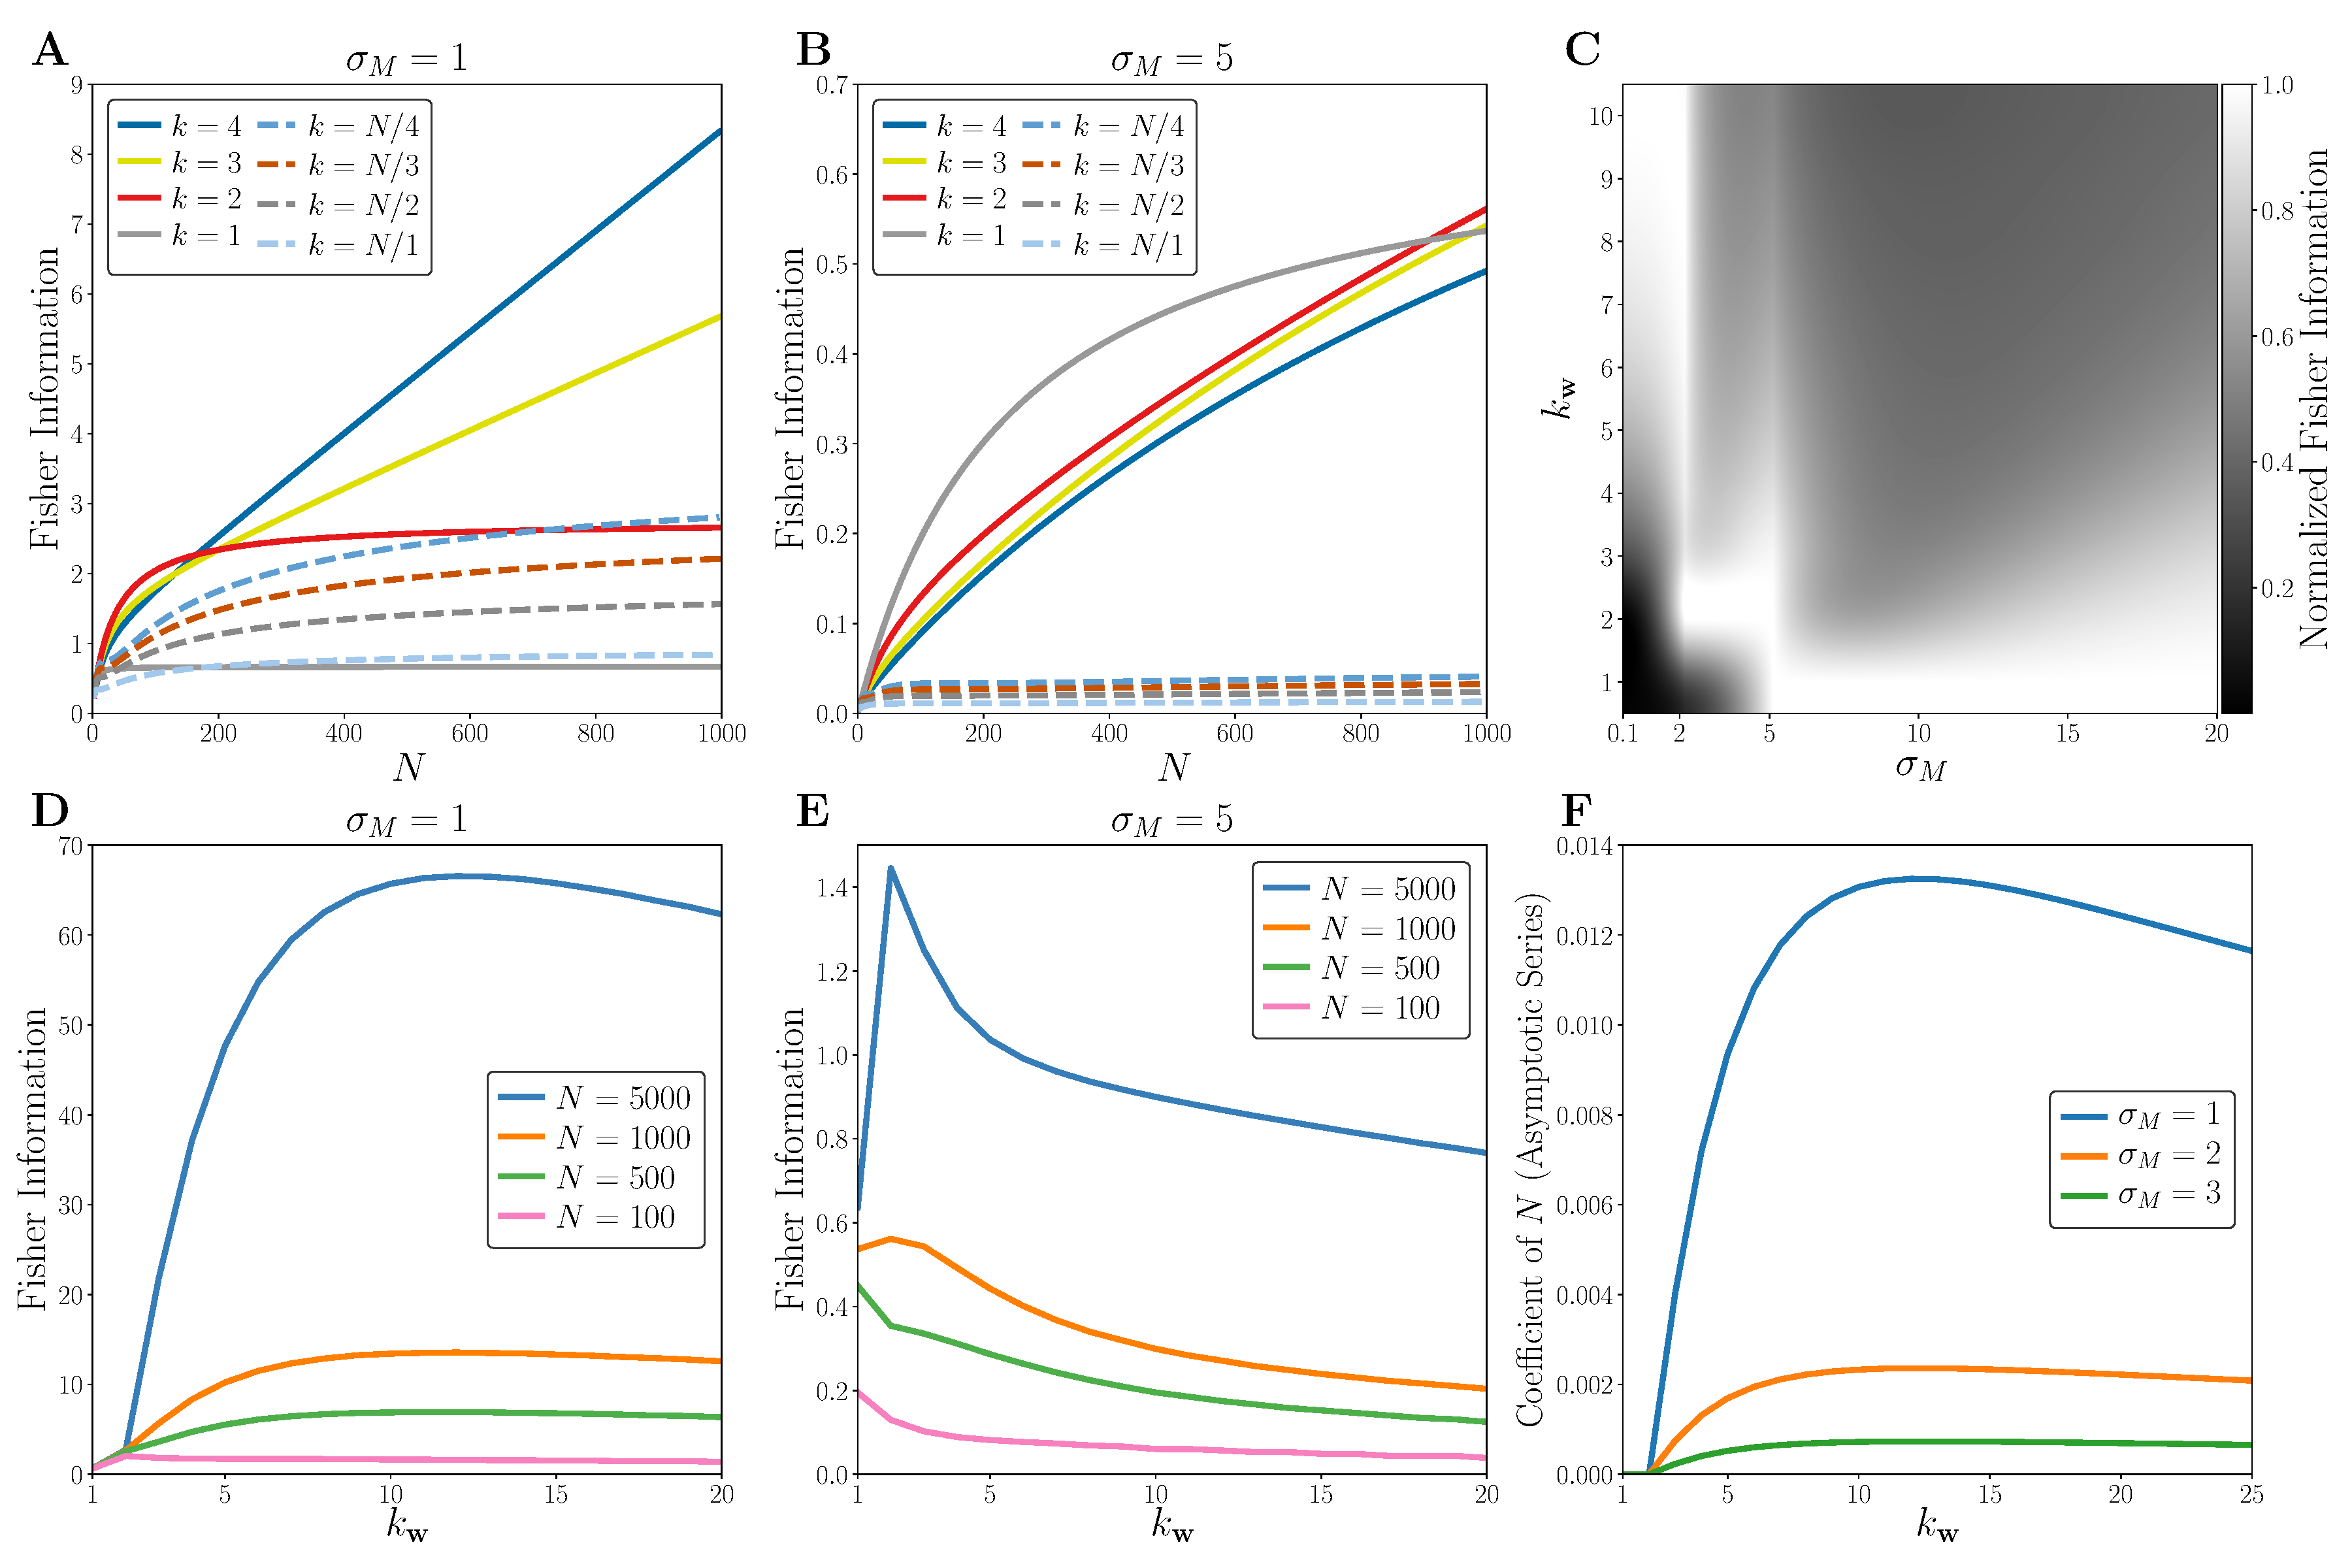
\includegraphics{img/figure3.pdf}}
		\caption{Fisher information in the network after a squared nonlinearity for structured weights. \textbf{(A)} When the membrane noise variance is equal to the common noise variance, we observe saturating behavior for $k=1$ and $k=2$. Increasing $k$ results in unbounded growth. At the extreme end of heterogeneity, where $k$ scales as $N$, the Fisher information saturates. \textbf{(B)} This qualitative behavior depends on the choice of $\sigma_P$. Increasing the membrane noise variance requires a much larger neural population to see the benefits of larger heterogeneity. \textbf{(C)} The Fisher information is normalized across all values of $\sigma_P/\sigma_C$ for a choice of $k$. The behavior of the Fisher information exhibits several phase transitions. This qualitative behavior may change as $N$ is increased.}
		\label{fig:fisher-quadratic}
	\end{figure}
	
	\subsubsection{Fisher Information}
	An analytic expression of the linear Fisher information is calculated in Appendix \ref{app:fisher-quadratic}. Its analytic form is too complicated to be restated here, but we will examine it numerically for both the structured and unstructured weights. The qualitative behavior of the Fisher information is dependent on the magnitude of the common ($\sigma_C$) and private ($\sigma_P$) variabilities, though not through their ratio $\sigma_C/\sigma_P$ (as in the linear stage). Thus, we separately consider how common and private variability impact coding efficacy under various synaptic weight structures.
	
	As before, we first turn to the structured weights with $k_{\mathbf{v}}=1$ and varying $k_{\mathbf{w}}$. First, consider $\sigma_P= \sigma_C=1$ (Figure \ref{fig:fisher-quadratic}A): here, the Fisher information saturates for both $k_{\mathbf{w}}=1$ and $k_{\mathbf{w}}=2$, but increases without bound for larger $k_{\mathbf{w}}$. We can also consider the other extreme, where $k_{\mathbf{w}}\sim O(N)$; in this case the Fisher information drastically decreases and  appears to saturate (Figure \ref{fig:fisher-quadratic}A, dashed lines). 
	
	At the extreme where private variability dominates, we see qualitatively different finite network behavior ($\sigma_P=5$, Figure \ref{fig:fisher-quadratic}B). For  $N=1000$,  both $k_{\mathbf{w}}=1$ and $k_{\mathbf{w}}=2$ exhibit better performance relative to larger values of $k_{\mathbf{w}}$ (meanwhile, $k_{\mathbf{w}} \sim O(N)$  quickly saturates). We note that, unsurprisingly, the increase in private variability has decreased \textit{all} Fisher informations compared to $\sigma_P=1$ (compare the scales of Figure \ref{fig:fisher-quadratic}A, B): our main interest is highlighting the optimal synaptic weighting \textit{given} some amount of private and common variability. Lastly, it is important to point out that Figure \ref{fig:fisher-quadratic} only highlights finite network behavior; indeed, as we will see, the asymptotic behavior is consistent no matter the choice of $\sigma_P$.
	
	Thus, the introduction of the squared nonlinearity produces qualitatively different behavior at the finite network level: in contrast with Figure \ref{fig:struct-linear}, increased heterogeneity does not automatically imply improved decoding. Indeed, there is a regime in which increased heterogeneity improves Fisher information, beyond which we see a reduction in decoding performance (Figure \ref{fig:fisher-quadratic}D). If the private variability increases, this regime shrinks or becomes nonexistent, depending on the network size (Figure \ref{fig:fisher-quadratic}E). Furthermore, entering this regime for higher private variability requires smaller $k_{\mathbf{w}}$. 
	
	The results shown in Figure \ref{fig:fisher-quadratic}D, E imply that there exists an interesting relationship between the network's decoding ability, its private variability, and its synaptic weight heterogeneity $k_{\mathbf{w}}$. To explore this further, we examined the behavior of the Fisher information at a finite network size ($N=1000$) as a function of both $\sigma_P$ and $k_{\mathbf{w}}$ (Figure \ref{fig:fisher-quadratic}C).  To account for the fact that an increase in private variability will always decrease the Fisher information, we calculate the \textit{normalized} Fisher information: for a given choice of $\sigma_P$, each Fisher information is divided by the maximum across a range of $k_{\mathbf{w}}$. Thus, a normalized Fisher information allows us to determine what level of synaptic weight heterogeneity maximizes coding fidelity, given a private variability $\sigma_P$.
	
	Figure \ref{fig:fisher-quadratic}C highlights three interesting regimes. When the private variability is small, the network benefits from larger weight heterogeneity on the common noise. But as our neurons become more noisy, the ``Goldilocks zone'' for which our network can leverage larger noise weights becomes constrained. When the private variability is large, our network is better off having less heterogeneous weights, despite the threat of induced differential correlations from the common noise. Between these regimes, there are transitions for which many choices of $k_{\mathbf{w}}$ result in equally good decoding performance.
	
	Lastly, we validated the asymptotic behavior of the Fisher information as a function of the private noise by examining the coefficient of $N$ in its asymptotic series (Figure \ref{fig:fisher-quadratic}F). For $k_{\mathbf{v}}=1,2$, the coefficient is zero for any choice of $\sigma_P$, implying that the Fisher information always saturates. In addition, when $k_{\mathbf{w}}\sim O(N)$, the asymptotic series is always sublinear (not shown in Figure \ref{fig:fisher-quadratic}F). Thus, there are multiple cases in which the structure of synaptic weighting can induce differential correlations in the presence of common noise. Increasing the heterogeneity allows the network to escape these induced differential correlations and achieve linear asymptotic growth. If $k_{\mathbf{w}}$ becomes too large, however, the linear asymptotic growth begins to decrease; once $k_{\mathbf{w}}$ scales as the population science, differential correlations are once again induced.
	
	\begin{figure}[t]
		\centering
		\scalebox{0.23}{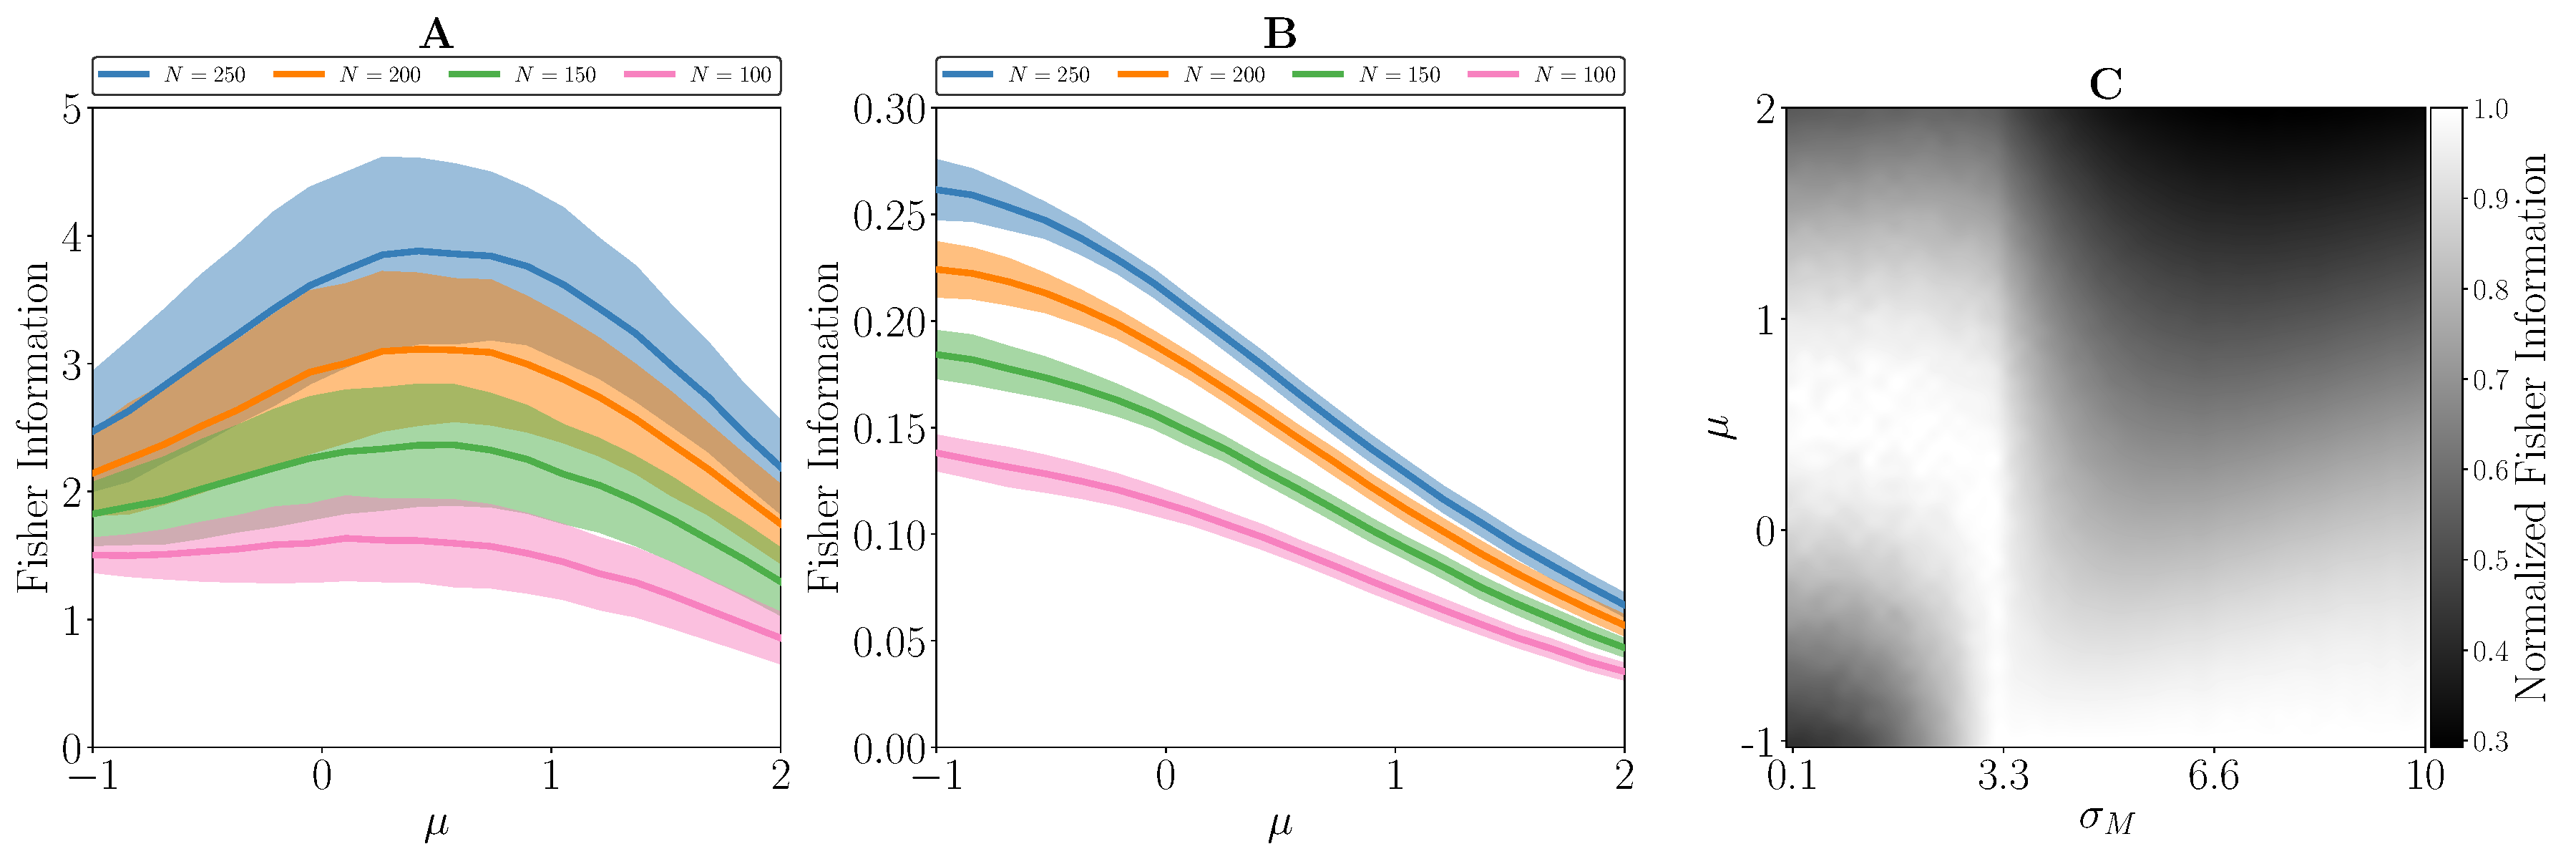
\includegraphics{img/figure4.pdf}}
		\caption{Linear Fisher information for unstructured weights under the presence of a quadratic linearity. \textbf{(A),(B)} } 
		\label{fig:unstructured-quadratic-fisher}
	\end{figure}
	
	\subsubsection{Unstructured Weights}
	We reproduced the above analysis with unstructured weights. As before, we drew   1000 samples of common noise weights from a shifted lognormal distribution with varying $\mu$. The behavior of the average (linear) Fisher information is qualitatively similar to that of the structured weights. There exists a regime for which larger weight heterogeneity improves the decoding performance, after which coding fidelity decreases (Figure \ref{fig:unstructured-quadratic-fisher}A). If the private noise variance dominates, this regime begins to disappear for smaller networks (Figure \ref{fig:unstructured-quadratic-fisher}B). Thus, when private noise dominates, the network is better off having less heterogeneous (and therefore, smaller) weights.
	
	To summarize these results, we once again plot the normalized Fisher information (this time, normalized across choices of $\mu$ and averaged over 1000 samples from the lognormal distribution) for a range of private variabilities (Figure \ref{fig:unstructured-quadratic-fisher}C).  The heat map exhibits a similar ``phase transition'' at a specific private variability. At this phase transition, a wide range of $\mu$'s provide the network with similar decoding ability. For smaller $\sigma_M$, we see behavior comparable to Figure \ref{fig:unstructured-quadratic-fisher}A, where there exists a regime of improved Fisher information. Beyond the phase transition, the network prefers less diverse synaptic weighting (though it becomes less stringent as $\sigma_M$ increases). The behavior exhibited by this heat map is similar to Figure \ref{fig:fisher-quadratic}C, but less complicated. 
	
	\subsection{Mutual Information}
	When the network possesses a quadratic nonlinearity, the mutual information $I[s,\mathbf{r}]$ is not analytically tractable. Therefore, we calculated the mutual information numerically on data simulated from the network, using an estimator built on $k$-nearest neighbor statistics \cite{kraskov}. We refer to this estimator as the KSG estimator. 
	
	We applied the KSG estimator to 100 unique datasets, each containing 100,000 samples drawn from the linear-nonlinear network. We then estimated the mutual information by averaging across each of the 100 estimators. The computational bottleneck for the KSG estimator lies in finding nearest neighbors in a kd-tree, which becomes prohibitive for large dimensions (around 20), so we considered much smaller network sizes than in the case of Fisher information. Furthermore, our estimator encountered difficulties when samples became too noisy, so we limited ourselves to smaller values of $(\sigma_M, \sigma_C)$.
	
	\subsection{The benefits of increased heterogeneity}
	Why are we afforded improved encoding and decoding as the common noise is amplified for certain neurons in the network? An increase in heterogeneity, as we have defined it, ensures that the common noise is magnified in the network. At the same time, however, the structure of the correlated variability induced by the common noise changes with increased heterogeneity. 
	
	At the linear stage, the answer appears to be clear: an increase in heterogeneity
	
	The network effective
where $\Delta$ sets a lower bound for the weights. Here, increased ``diversity'' in the sense of the structured weights is achieved by increasing $\mu$, which increases the mean, median, and mode of the lognormal distribution. This is in contrast with increasing $\sigma$, which will decrease the mode of the distribution.




\section*{Conclusion}
We have illustrated the basic format to the manuscript that you consider to submit to Neural Computation. We hope this is helpful to the authors.

\subsection*{Acknowledgments}


\section*{Appendix}

\subsection{Calculation of  Fisher Information, Linear Stage}
All variability after the linear stage is Gaussian; thus, the Fisher information can be expressed in the form \citep{abbott1999, kay1993}:
\begin{align}
	I_{F}(s) &= \mathbf{f}'(s)^T \boldsymbol{\Sigma}^{-1} (s) \mathbf{f}'(s) + \frac{1}{2}\Tr\left[\boldsymbol{\Sigma}'(s) \boldsymbol{\Sigma}^{-1}(s)\boldsymbol{\Sigma}'(s) \boldsymbol{\Sigma}^{-1}(s)\right]. \label{IF-gaussian}
\end{align}
Our immediate goal is to calculate $\mathbf{f}(s)$, the average response of the linear stage, and $\boldsymbol{\Sigma}$, the covariance between the responses. The output of the $i$th neuron after the linear stage is
\begin{align}
	\ell_i &= v_i s + w_i \sigma_C \xi_C + \sigma_P\xi_{P,i},
\end{align}
so that the average response as a function of $s$ is
\begin{align}
	f_i(s) &= \langle \ell_i \rangle = v_i s.
\end{align}
Thus,
\begin{align}
	\mathbf{f}(s) = \mathbf{v}s \Rightarrow \mathbf{f}'(s) = \mathbf{v}.
\end{align}
Meanwhile,
	\begin{align}
	\langle \ell_i \ell_j \rangle &= \langle (v_i s + w_i \sigma_C\xi_C + \sigma_P\xi_{P,i}) (v_j s + w_j \sigma_C\xi_C + \sigma_P\xi_{P,j})\rangle \\
	&= v_i v_j s^2 + w_i w_j \sigma_C^2 + \sigma_P^2 \delta_{ij}
	\end{align}
	so that
	\begin{align}
	\Sigma_{ij} &= v_i v_j s^2 + w_i w_j \sigma_C^2 + \sigma_P^2 \delta_{ij} - v_i v_j s^2 \\
	&= \sigma_P^2 \delta_{ij} + w_i w_j \sigma_C^2 \\
	\Rightarrow \boldsymbol{\Sigma} &= \sigma_P^2 \mathbf{I} + \sigma_C^2\mathbf{ww}^T.
	\end{align}
	Notice that the covariance matrix does not depend on $s$, so the second term in equation \eqref{IF-gaussian} will vanish. We do, however, need the inverse covariance matrix for the first:
	\begin{align}
	\boldsymbol{\Sigma}^{-1} &= \frac{1}{\sigma_P^2} \mathbf{I} - \frac{\sigma_C^2}{\sigma_P^4} \frac{\mathbf{ww}^T}{1+\frac{\sigma_C^2}{\sigma_P^2}||\mathbf{w}||^2}\\
	&= \frac{1}{\sigma_P^2}\left(\mathbf{I} - \frac{\sigma_C^2}{\sigma_P^2 + \sigma_C^2 |\mathbf{w}|^2}\mathbf{ww}^T\right).
	\end{align}
	Hence, the Fisher information is
	\begin{align}
	I_{F}(s) &= \frac{1}{\sigma_P^2}\mathbf{v}^T \left(\mathbf{I} - \frac{\sigma_C^2}{\sigma_P^2 + \sigma_C^2 |\mathbf{w}|^2}\mathbf{ww}^T\right) \mathbf{v} \\
	&= \frac{1}{\sigma_P^2} \left(|\mathbf{v}|^2 - \frac{\sigma_C^2 (\mathbf{v}\cdot\mathbf{w})^2}{\sigma_P^2 + \sigma_C^2 |\mathbf{w}|^2}\right) \\
	&= \frac{1}{\sigma_P^2}\frac{\left(\sigma_P^2/\sigma_C^2\right) |\mathbf{v}|^2 +  \left(|\mathbf{v}|^2|\mathbf{w}|^2 - (\mathbf{v}\cdot\mathbf{w})^2\right)}{(\sigma_P^2/\sigma_C^2)+ |\mathbf{w}|^2}.
	\end{align}

\begin{thebibliography}{100}
\providecommand{\natexlab}[1]{#1}
\expandafter\ifx\csname urlstyle\endcsname\relax
  \providecommand{\doi}[1]{doi:\discretionary{}{}{}#1}\else
  \providecommand{\doi}{doi:\discretionary{}{}{}\begingroup
  \urlstyle{rm}\Url}\fi

\bibitem[{Abbott \& Dayan(1999)}]{abbott1999}
Abbott, L. F., \& Dayan, P. (1999).
\newblock The Effect of Correlated Variability on the Accuracy of a Population Code.
\newblock \emph{Neural Computation}, \emph{1}, 91--101.

\bibitem[{DeWeese \& Zador(2004)}]{deweese2004}
DeWeese, M. R., \& Zador, A. M. (2004).
\newblock Shared and Private Variability in the Auditory Cortex.
\newblock \emph{J. Neurophysiol.}, \emph{92}, 1840--1855.

\bibitem[{Kay(1993)}]{kay1993}
Kay, S. M. (1993).
\newblock Fundamentals of Statistical Signal Processing, Volume I: Estimation Theory.
\newblock \emph{Prentice-Hall}.

\bibitem[{Authors et~al.(2008)Author1, Author2, \&
  Author3}]{Ref2008}
Author1, A., Author2, A., \& Author3, A. (2008).
\newblock Title for the second reference.
\newblock \emph{Journal for the second reference}, \emph{5}, 188 -- 200.

\end{thebibliography}
\end{document}